% ADD ./styles DIRECTORY TO TEXINPUTS AND BSTINPUTS!!!!

\documentclass[a4paper,11pt,oneside]{article}
\usepackage[american]{babel}			% American hyphenation
\usepackage[latin1]{inputenc}			% Recognizes special characters (accented letters, etc.)
\usepackage[pdftex]{graphicx}			% Allows the use of images through \includegraphics
\DeclareGraphicsExtensions{.pdf, .png, .jpg, .gif, .bmp}
\usepackage{verbatim}				% Allows the use of the comment environment
\usepackage{paralist}				% Allows the use of inparaenum
\usepackage{algorithm2e}			% Allows the use of the algorithm environment
\usepackage[amssymb]{SIunits}			% Allows to use the symbols for SI units
\usepackage{numprint}				% Allows to use advanced formatting for numbers
\usepackage{amsthm}				% Allows the use of the defn environment
\usepackage{amsmath}				% Introduces advanced mathematical notations
\usepackage{amssymb}				% Introduces various math symbols
%\usepackage{wasysym}				% Introduces the WASY symbols
\usepackage{bibentry}				% BibTeX

\usepackage{fancyhdr}				% Introduces the Fancy style
\usepackage[pdftex,plainpages=false,pdfpagelabels,colorlinks,linkcolor=black,citecolor=black,filecolor=black,urlcolor=black]{hyperref}
% Introduces the hypertextual references on the document. THIS SHOULD BE THE LAST INSERTED PACKAGE!

\setlength{\headheight}{15pt}			% Sets the height of the header
\setlength{\parindent}{5mm}			% Sets the indentation of new paragraphs
\linespread{1.2}				% Sets the line height
\makeindex					% Starts the collection of the words between \index{} to create the Index

\begin{document}

\hypersetup{pdfauthor={Fabio Arlati and Antonio Miele},pdftitle={PacketNoc - How To}}
\hypersetup{bookmarksopen}			% Sets author, title, and options in the PDF properties
\pagenumbering{arabic}				% Numeric page numbers
\fancyhead{}
\fancyfoot{}
\fancyhead[OR]{\slshape \leftmark}
\fancyhead[OL]{}
\fancyfoot[OC]{\thepage}
\pagestyle{fancy}				% (above and this) Sets the style 'fancy' for the text

\title{\Huge \textit{\textsc{PacketNoc - How To}}}
\author{Fabio Arlati - \href{mailto:arlati.fabio@gmail.com}{arlati.fabio@gmail.com} \\ Antonio Miele - \href{mailto:miele@elet.polimi.it}{miele@elet.polimi.it}}
\date{First draft: July 2010\\ Revision: October 2010}
\maketitle					% This and the commands above are used to make the original LaTeX title

\tableofcontents
%\listoffigures

\section*{What is this document?}
This document is an hands-on guide to the use of the packet NOC component defined in ReSP. The instantiation, connection and manipulation of this component will be described in the next few sections with the aid of some pictures.

\section{Definition}
\label{def}
This NOC model is a standard TLM component (which could be attached to other elements in ReSP), but is internally built as a common SystemC component that represents a set of packet-exchanging components. In particular, the internal architecture of the NOC model is based upon three different types of components:
\begin{enumerate}
  \item Master Processing Element (MPE), which represents the interface module between a connected master and the NOC. It is devoted to the pa\-cketing the TLM transactions coming from the attached TLM initiator;
  \item Switch, which receives, memorizes into a buffer, and forwards the packets according to a given route;
  \item Slave Processing Element (SPE), which represent the interface module between a connected slave and the NOC. It is devoted to unpacket TLM tran\-sactions, forward them to the attached TLM target, and send back a packeted answer to the requesting MPE.
\end{enumerate}
For every TLM transaction, the appropriate MPE starts a new session (co\-mposed by one or more packets). This session is concluded only when the entire answer (composed, in turn, by one or more packets) is received from the SPE. If the answer is not received before a fixed timeout, the session is restarted, and a new series of requesting packets is created by the MPE. Until a session has not been successfully completed, the TLM transaction will not be concluded.

\section{Instantiation}
\label{inst}
A simple example of how a packet NOC can be instantiated is contained in the following ReSP architecture file:
\begin{verbatim}
  resp-sim/architectures/test/test_packetNoc.py
\end{verbatim}
As shown in Figure \ref{inst:code} at lines at lines 132-133, the NOC is instantiated starting from a small set of parameters:
\begin{itemize}
  \item A name for the component (\textit{noc} in the example).
  \item The path to an \texttt{xml} file describing the NOC (contained in the NOC\_ DESCRIPTION variable of the example).
  \item The period of the internal clock of the NOC (calculated starting from the NOC\_FREQUENCY variable of the example).
\end{itemize}

\begin{figure}[htbp]
\begin{center}
  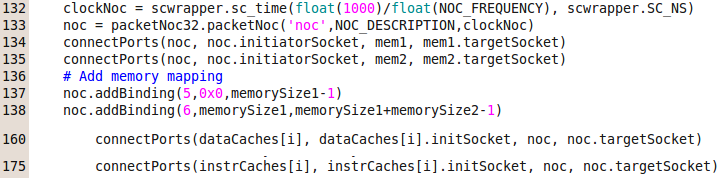
\includegraphics[width=0.9\textwidth]{instantiation}
\end{center}
\caption{The instantiation of NOC  example}
\label{inst:code}
\end{figure}

The following \texttt{xml} file describes the NOC of the considered example:
\begin{verbatim}
  resp-sim/architectures/test/test_packetNoc.xml
\end{verbatim}
Figure \ref{inst:xml} shows a fragment of the XML descriptor.
The XML descriptor has to contain a number of MPEs equal to the number of initiator components we want to connect; similarly, it has to contain a number of SPEs equal to the number of target components we want to connect. 
In the considered, the architecture is composed by 4 master components (2 processors, which, according to the Harvard architecture, have both a data and an instruction port) and 2 slave components (2 simple memories). Thus, inside the NOC XML descriptor we need to declare 4 MPEs and 2 SPEs; moreover, every MPEs and SPEs require a unique ID as an attribute. 
Between these elements we are free to declare an undefined number of switches with any kind of topology: even the switches require a unique ID attribute. The connections can be declared through the \textit{connect} tag embedded inside an element, specifying the target ID; connections are unidirectional, thus for a bidirectional path it is necessary to specify another 
\textit{connect} tag for the inverse direction. The number of connections is limited in the following ways:
\begin{itemize}
  \item Processing elements are allowed to have only one connection.
  \item Switches can have up to \textit{PORTS} connections, where \textit{PORTS} is a constant defined in \texttt{/resp-sim/components/interconnection/\linebreak packetNoc/nocCommon.hpp}. Moreover, at most a MPE or a SPE can be connected to each switch. The standard value of \textit{PORTS} is 5, if you want to modify it, you should recompile the tool (use \texttt{./waf} in the main folder).

\end{itemize}
\begin{figure}[tbp]
\begin{center}
  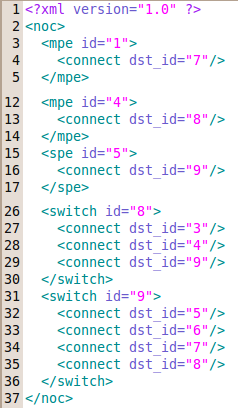
\includegraphics[width=0.3\textwidth]{xml}
\end{center}
\caption{The XML descriptor of NOC example}
\label{inst:xml}
\end{figure}

Starting from this information the entire NOC is initialized, the SystemC connections between the components are automatically performed, and the routing tables of the switches are automatically computed by applying the Dijkstra algorithm to an ad-hoc Boost Graph. Figure~\ref{xml:graph} shows the graph obtained by reading the file in our example.

\begin{figure}[htbp]
\begin{center}
  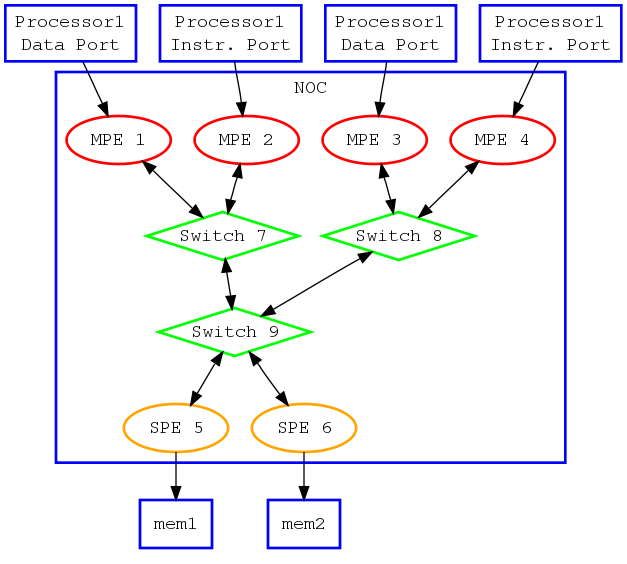
\includegraphics[width=0.6\textwidth]{graph}
\end{center}
\caption{The connection graph of the NOC example}
\label{xml:graph}
\end{figure}

After the instantiation, the NOC is connected to the initiator components (the masters, usually the processors and their caches), at lines 160 and 175 and to the target components (the slaves, usually the memories) at lines 134-135. 
Keep in mind that the NOC externally provides only two multi passthrough TLM ports (one for targets and one for initiators); then, internally the various initiator and target components are binded to the appropriate MPE or SPE according to a positional order of the components' connection and MPEs/SPEs' declaration. For instance, first connected initiator port, that is the data port of the first processor is connected to MPE 1 that is the first MPE defined in the XML file, and so on; similarly, \textit{mem1} is binded to SPE 5 and \textit{mem2} is binded to SPE 6.

% every TLM connection assigned to the ports through the \texttt{connectPorts} command is identified by an index, which is used to access the correct port as in a common array. This index starts from 0 and is automatically incremented for every connection. 

Finally, we have to define the map the various target components in the address space. it is performed at lines 137-138 where the first parameter represents the ID of the SPE of the target component we want to map.

\section{Interaction}
\label{inter}
The NOC provides a complete set of functions to monitor and modify its behavior at run-time:
\begin{description}
\item[printBindings()] prints on the standard output the address bindings of the NOC.
\item[printGRT()] prints on the standard output all the Routing Tables of the NOC switches.
\item[printStats()] prints on the standard output all the current statistics of the NOC elements (flits received, sent and dropped).
\item[getActivePorts(unsigned int switchId)] returns the IDs of the active ports in a given switch.  
\item[getBufferCurrentFreeSlots(unsigned int switchId, unsigned int portId)] returns the number of free slots in a specific buffer of a switch.
\item[getFlitsIn(unsigned int elId, unsigned int portId)] returns the number of flits received by a particular element on a specific port. In case the element is a MPE or a SPE, portId is ignored.
\item[getFlitsOut(unsigned int elId, unsigned int portId)] returns the number of flits sent by a particular element on a specific port. In case the element is a MPE or a SPE, portId is ignored.
\item[getTimeouts(unsigned int masterId)] returns the number of sessions timed out in a particular master element.
\item[getAllTimeouts()] returns the number of sessions timed out in all master elements.
\item[getBufferSize(unsigned int switchId, unsigned int portId)] returns the size of a specific buffer of a given switch.
\item[getDropped(unsigned int switchId, unsigned int portId)] returns the number of flits dropped by a particular switch on a specific port.
\item[getAllDropped()] returns the number of flits dropped by all the switches.
\item[changeTimeout(unsigned int masterId, sc\_time tO)] changes the timeout value of a particular master element. The standard timeout is 100 \nano\second, and is hardcoded in \texttt{/resp-sim/components/interconnection/\linebreak packetNoc/nocCommon.hpp}. If you wish to change the standard timeout, you should reissue \texttt{./waf} in the main folder.
\item[changeAllTimeouts(sc\_time tO)] changes the timeout value of every master element.
\item[changeBufferSize(unsigned int switchId, unsigned int portId, unsigned int size)] changes the size of specified buffer of a particular switch. The standard buffer size if 1, and is hardcoded in \texttt{/resp-sim/components/interconnection/\linebreak packetNoc/nocCommon.hpp}. If you wish to change the standard buffer size, you should reissue \texttt{./waf} in the main folder.
\item[changeAllBufferSizes(unsigned int size)] changes the buffer size of e\-very switch.
\item[changePath(unsigned int switchId, unsigned int destinationId, unsigned int nextHop)] changes the forwarding path for a given destination in a particular switch. The \texttt{nextHop} parameter requires the ID of a switch (or an element) directly attached to the switch under analysis. The forwarding paths are initialized by the Dijkstra shortest path algorithm applied to the network graph when the NOC is constructed.
\item[getSwitchIds()] returns the list of the IDs of all the switches instantiated in the NOC.
\end{description}
An example of how these functions are used can be found in \texttt{resp-sim/\linebreak architectures/test/test\_packetNoc.py} at line 223, where all the timeouts of the master elements are set to 1 \micro\second. This operation is necessary in our example, because whenever one of the caches requires to load an entire block of memory, a huge amount of packets is generated during the session; in order to allow the completion of these sessions, a greater timeout is required in the master elements, otherwise every session will reach the standard timeout of 100 \nano\second. It is strongly recommended to use this approach to change the standard parameters of the NOC, instead of modifying the constants in \texttt{nocCommon.hpp}.

It is worth noting that the described interface can be easily enhanced in order to expose further methods for accessing and modifying the NOC characteristics.

\section{Automatic Interaction}
\label{autointer}
It is possible to instantiate a particular component, named \textit{governor}, which automatically executes a specified routine every specified period of time. This governor is directly attached to the packet NOC, thus it is possible to perform an automated interaction using the functions specified in Section~\ref{inter}.

The governor can be instantiated as shown in \texttt{resp-sim/\linebreak architectures/test/test\_packetNoc2.py} at line 102. It requires three parameters:
\begin{itemize}
  \item A name for the component (\textit{governor} in the example).
  \item The NOC object previously instantiated (\textit{noc} in the example).
  \item The period of the internal clock of the governor (1 \milli\second~in the example).
\end{itemize}

The behavior of the governor is simple: at every clock cycle (i.e. every \milli\second), a routine is executed: this routine is named \texttt{activity} and is specified in \texttt{resp/components/interconnect/packetNoc/governor/packetNocGover\linebreak nor.cpp}.
The user can customize the routine simply by re-implementing the function body. remember that, after the routine has been changed, a recompilation should be issued by launching \texttt{./waf} in the main folder.
 
In the example proposed in \texttt{resp-sim/architectures/test/test\linebreak \_packetNoc2.py}, the \texttt{activity} routine implements a simple resource manager able to dynamically reconfigure the sizes of the buffers inside each switch according to the information about the traffic in the NOC. In particular, the memory slots are distributed among the buffers of each switch according to the packet drop statistics; in this way, the size of the buffers on on the direction the switch is experiencing a higher traffic are increased with the free slots of the buffers on the other directions.

The governor is initialized at lines 94-104 of the architecture file by specifying a set of parameters:
\begin{enumerate}
\item[BUFFER\_SIZE] the initial buffer size;
\item[INIT\_THRESHOLD] the initial value of the parameter driving the buffer size changing;
\item[MIN\_THRESHOLD] the minimum threshold for the parameter driving the buffer size changing;
\item[MAX\_THRESHOLD] the maximum threshold for the parameter driving the buffer size changing;
\item[MULT\_FACTOR] a multiplication factor used on packet drop;
\item[RED\_FACTOR] a reduction factor used when no packet drop occurs on a specific buffer
\end{enumerate}
Given these parameters, the \textit{activity} algorithm works as following: a \textit{drop\_index} parameter is assigned to every buffers of each switch and it is initialized with \textit{INIT\_THRESHOLD} value. At each execution of the \textit{activity} routine, each buffer of each switch is checked to detect if any drop occurred. For each occurred drop, \textit{drop\_index} is multiplied by MULT\_FACTOR; otherwise, it is subtracted by RED\_FACTOR. Then, if \textit{drop\_index} of a buffer overcomes the \textit{MAX\_THRESHOLD}, its size is increased by one by removing a slot from another buffer of the same switch with the minimum \textit{drop\_index} (it should have at least a free slot); after, the \textit{drop\_index}s of both the buffers are re-initialized. Similarly, if a buffer \textit{drop\_index} becomes lower than \textit{MIN\_THRESHOLD} and it has a free slot, the slot is reassigned to another buffer of the same switch with the highest \textit{drop\_index} and the two parameters are re-initialized. In this way, it is possible to note that when accurately tuning the parameters, there is a reduction in the packets' drop and consequently in the overal execution time.
Another example of use of the \textit{governor} is shown in the architecture \texttt{resp-sim/architectures/test/test\linebreak \_packetNoc3.py}.

\end{document} 